\documentclass[tikz,border=2pt]{standalone}
\usepackage{amsmath,amssymb}
\usepackage{pgfplots}
\pgfplotsset{compat=1.18}

\begin{document}
% Density 2 on 0 < x < y < 1, observation X = 0.4. Prior f_Y(y) = 2y, likelihood
% f_{X|Y}(0.4 | y) = 1/y for y > 0.4; their product is constant, so the posterior is
% uniform on (0.4, 1) with height 1/(1 - 0.4).
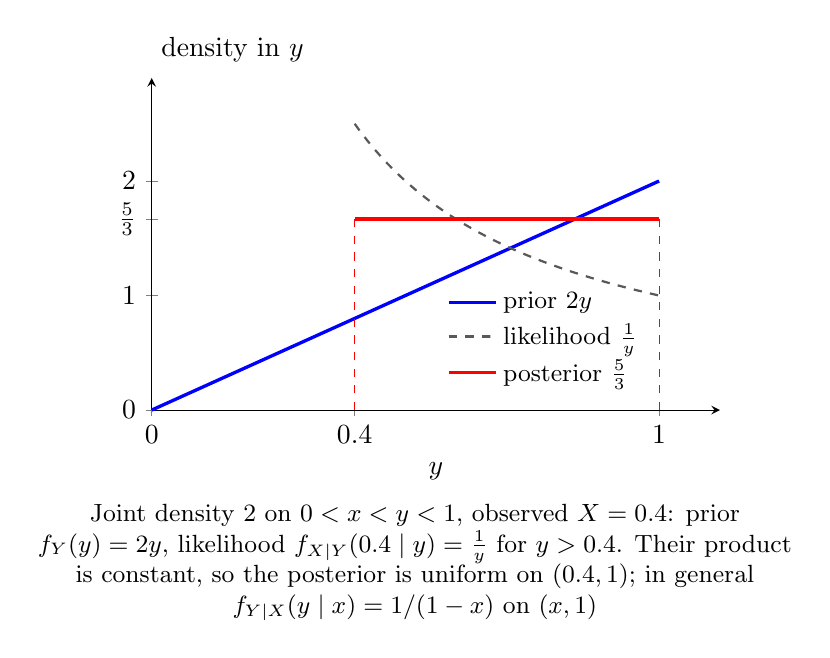
\begin{tikzpicture}
	\begin{axis}[
		axis lines=left, xmin=0, xmax=1.12, ymin=0, ymax=2.9,
		xtick={0,0.4,1}, ytick={0,1,1.667,2}, yticklabels={$0$,$1$,$\tfrac53$,$2$},
		xlabel={$y$}, ylabel={density in $y$}, ylabel style={rotate=-90, anchor=south west, at={(axis description cs:0,1.02)}},
		samples=100, smooth, width=8.8cm, height=5.8cm, clip=false,
		legend style={draw=none, fill=none, font=\small, at={(0.88,0.04)}, anchor=south east}, legend cell align=left
		]
		\addplot[blue, very thick, domain=0:1] {2*x};
		\addlegendentry{prior $2y$}
		\addplot[gray!70!black, thick, dashed, domain=0.4:1] {1/x};
		\addlegendentry{likelihood $\tfrac1y$}
		\addplot[red, very thick] coordinates {(0.4,1.667) (1,1.667)};
		\addlegendentry{posterior $\tfrac53$}
		\draw[red, dashed] (axis cs:0.4,0) -- (axis cs:0.4,1.667);
		\draw[red, dashed] (axis cs:1,0) -- (axis cs:1,1.667);
	\end{axis}
	\node[anchor=north, font=\small, align=flush center, text width=9.6cm] at ([yshift=-2pt]current axis.outer south) {Joint density $2$ on $0<x<y<1$, observed $X=0.4$: prior $f_Y(y)=2y$, likelihood $f_{X\mid Y}(0.4\mid y)=\tfrac1y$ for $y>0.4$. Their product is constant, so the posterior is uniform on $(0.4,1)$; in general $f_{Y\mid X}(y\mid x)=1/(1-x)$ on $(x,1)$};
\end{tikzpicture}
\end{document}
